\section{CONTOUR3 3D Contour Plot Function}

\subsection{Usage}

This command generates contour plots where the lines are plotted in 3D.
The syntax for its use is identical to the \verb|contour| function.  Please
see its help for details.
\subsection{Example}

Here is a simple example of a 3D contour plot.
\begin{verbatim}
--> [x,y] = meshgrid([-2:.25:2]);
--> z=x.*exp(-x.^2-y.^2);
--> contour3(x,y,z,30);
Warning: Newly defined variable xlim shadows a function of the same name.  Use clear xlim to recover access to the function
Warning: Newly defined variable ylim shadows a function of the same name.  Use clear ylim to recover access to the function
Warning: Newly defined variable zlim shadows a function of the same name.  Use clear zlim to recover access to the function
--> axis square;
--> view(-15,25)
Warning: Newly defined variable xlim shadows a function of the same name.  Use clear xlim to recover access to the function
Warning: Newly defined variable ylim shadows a function of the same name.  Use clear ylim to recover access to the function
Warning: Newly defined variable zlim shadows a function of the same name.  Use clear zlim to recover access to the function
\end{verbatim}
The resulting plot


\centerline{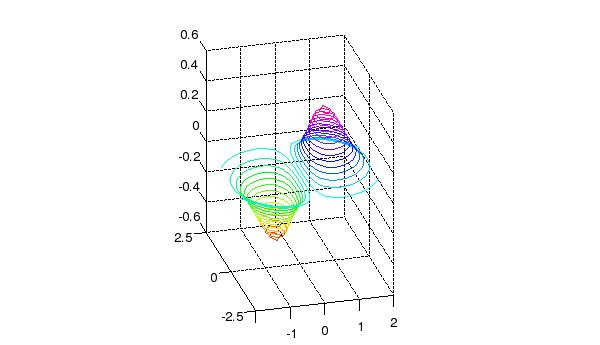
\includegraphics[width=8cm]{contour3_1}}

